\documentclass[sw]{iosart2c}
\usepackage[utf8]{inputenc}
\usepackage[T1]{fontenc}
\usepackage{times}
\usepackage{natbib}
\usepackage{amsmath}
\usepackage{dcolumn}
\usepackage{graphicx}
\usepackage{url}
\usepackage{xspace}
\usepackage{color}
\usepackage{eurosym}
\usepackage{todonotes}
\usepackage[breaklinks]{hyperref}
\def\sectionautorefname{Section}
\def\subsectionautorefname{Section}
\usepackage{multirow}
\usepackage{booktabs}
\usepackage{tabularx}
\usepackage{array}

%\usepackage{authblk}

\usepackage{textcomp}
\newcolumntype{R}{>{\raggedleft\arraybackslash}X}
\newcolumntype{L}{>{\raggedright\arraybackslash}X}
\newcolumntype{C}{>{\centering\arraybackslash}X}

\newcommand{\TODO}[1]{{\color{red}{\textbf{TODO: {#1}}\xspace}}}
\newcommand{\CONSIDER}[1]{{\color{blue}{\textbf{CONSIDER: {#1}}\xspace}}}
\newcolumntype{d}[1]{D{.}{.}{#1}}

\newcommand{\claus}[1]{\todo[inline]{[Claus: #1]}}
%\newcommand{\textrdf}[1]{\texttt{#1}}
\newcommand{\vocab}[1]{\emph{#1}}


\usepackage[scaled]{beramono}
\newcommand\Small{\fontsize{9}{9.2}\selectfont}
%\newcommand*\LSTfont{\Small\ttfamily\SetTracking{encoding=*}{-60}\lsstyle}


\usepackage{listings}
%\lstset{language=Python}
%\lstset{%
% morekeywords={Create,View,As,Construct,With,From}
%}%
\lstset{emph={%  
    Create,View,As,Construct,With,From%
    },emphstyle={\color{blue}\bfseries}%
}%



%\usepackage{verbatim}
\lstset{%
    numberbychapter=false,
    numbers=left,
    numberstyle=\tiny,
    basicstyle=\footnotesize\ttfamily,
    tabsize=2,
    framexleftmargin=2pt,
    captionpos=b,
    frame=single,
    breaklines=true
}
\lstdefinestyle{rdf}{numberblanklines=true, morekeywords={}}
\lstdefinestyle{sparql}{basicstyle=\ttfamily\scriptsize,numberblanklines=true,
    morekeywords={SELECT,OPTIONAL,FROM,DISTINCT,a,WHERE,FILTER,GROUP,ORDER,LIMIT,BY,IN,AS},
    emph={r,pub,aairObject,verb,person,bday,s,p,o},emphstyle=\textit
}
\lstdefinestyle{turtle}{basicstyle=\ttfamily\tiny ,numberblanklines=true,
    morekeywords={a, @prefix},
    morecomment=[s][\textrm]{<}{>},
    morecomment=[s][\textit]{"}{"},
}

% Default \todo{} to inline mode
\newcommand*{\origtodo}{}
\let\origtodo\todo
\renewcommand*{\todo}{\origtodo[inline]}




\firstpage{1} \lastpage{5} \volume{1} \pubyear{2012}
\begin{document}
\begin{frontmatter} 


%\pretitle{Pretitle}

\title{PanLex-RDF}
\runningtitle{Countering language attrition with the Web of Data}
%\todo{find a real title}

\review{Name Surname, University, Country}{Name Surname, University, Country}{Name Surname, University, Country}

%\author[1]{\fnms{Patrick} \snm{Westphal}},
%\author[1]{\fnms{Claus} \snm{Stadler}},
%\author[2]{\fnms{Jonathan} \snm{Pool}}
%\address[1]{University of Leipzig, Institute of Computer Science, AKSW}
%\address[2]{TODO}

%\address[1]{University of Leipzig, Institute of Computer Science, AKSW, Postfach 100920, D-04009 Leipzig, Germany}

%\author[A]{Patrick Westphal\thanks{A.A@university.edu}},
%\author[A]{Claus Stadler\thanks{cstadler@informatik.uni-leipzig.de}},
%\author[B]{Jonathan Pool\thanks{todo}}
%\address[A]{University of Leipzig, Institute of Computer Science, AKSW, Postfach 100920, D-04009 Leipzig, Germany\\ E-mail: \{lastname\}@informatik.uni-leipzig.de}
%\address[A]{University of Leipzig, Institute of Computer Science, AKSW, Postfach 100920, D-04009 Leipzig, Germany}
%\address[B]{TODO}

%\author[A]{\fnms{Patrick} \snm{Westphal}}
%\author[B]{\fnms{Claus} \snm{Stadler}}

%\runningauthor{M. Martin et al.}

%\address[B]{University of Leipzig}
%\address[C]{TODO}
%\todo{the e-mail address pattern won't work for both of us}

\begin{abstract}
At present, there are approximately 7,000 living languages in the world.
However, some experts claim that the process of globalization may eventually lead
to the world losing this linguistic diversity.
The vision of the PanLex project is to save these languages, especially low-density ones,
by allowing them to be intertranslatable and thus to be a part of the Information Age.
For this reason, PanLex gathers and integrates information from thousands of
linguistic resources, such as monolingual dictionaries, bilingual dictionaries, multilingual dictionaries,
glossaries, standards and thesauri.
In this paper we describe how we transformed this data to RDF, interlinked it with
lexvo and DBpedia and published it as Linked Data and SPARQL.
\end{abstract}

\begin{keyword}
Multi-lingual Linked Open Data, PanLex, Lexcial Resource, RDF, RDB2RDF, Sparqlify
\end{keyword}
\end{frontmatter}

\section{Introduction}
% \begin{itemize}
% \item introduce PanLex project
% \item @author: Jonathan
% \item Motivation: About approximately 6900 active languages (\todo{source seems to be http://www.amazon.com/Ethnologue-Languages-M-Paul-Lewis/dp/1556712162}), Existing translation only between relatively few language pairs (dictionaries).
% \item Transitive word-by-word translations 
% * high density and low density languages
% * decline in linguistic diversity
% * These combined forces have led to predictions that something between half and 90%
%   of the world's living languages will die within the next century (Woodbury 2006; UNESCO 2003: 2).
%   Weaker forms of these forces appear to be shrinking the use of medium-density languages in science,
%   diplomacy, business, and other domains (Phillipson 2008).
% * When languages die, they argue, the world loses
%   (1) irreplaceable knowledge of history, medicine, nature, and productive methods encoded in languages'
% * extraction + integration
% \end{itemize}
At present, there are about 7,000 living languages in the world\footnote{See \url{http://www.sil.org/iso639-3/download.asp} for a list of registered languages}.
Nonetheless, some experts claim that processes such as nation-state consolidation and globalization are producing language attrition so rapidly that up to 90\% of all languages alive today will be extinct within a century~\cite{endang_lang}.
Theorists of biolinguistic diversity argue that the loss of
language diversity, the loss of human biological knowledge, and the loss of
species diversity are mutually supportive and thus that language preservation
and revitalization are essential to the preservation of biological diversity~\cite{nettle}.
The vision of the PanLex project is to save all these thousands of languages,
especially those low-density ones that are threatened by extinction,
by supporting their use in global communication. This requires panlingual
translation: translation from any language of the world into any other.
One of the crucial components of panlingual translation of discourses is
panlingual lexical translation. PanLex is designed to support that component.
It documents the known lexical translations (translations of lexemes) among all
languages.
 
Although a list of all the translations of all words into all other languages
would be large (amounting to trillions of translations), there are more
serious obstacles. The vast majority of these translations are unknown.
Those that are known are not universally agreed on. And lexical polysemy
and ambiguity make the question ``What is the translation of lexeme X into language Y?''
underspecified for practical purposes.
So the PanLex project is designed to permit the application of artificial
intelligence techniques to infer and select translations.

Currently there is a growing community trying to combine linguistic knowledge
with Semantic Web technologies and thereby build a Web of Linguistic Data,
also known as the \emph{Linguistic Linked Open Data (LLOD) cloud}.
The PanLex project is still in its data-acquisition phase, but it has provided a
few web services\footnote{\url{http://panlex.org/try/}} and
APIs\footnote{\url{http://panlex.org/tech/doc/api/}} to access its data.
Since the project shares the idea of open access, we have undertaken the project
of making PanLex a part of the LLOD cloud.

In \autoref{sec:triplificate} we will introduce the PanLex dataset, present our
PanLex RDF vocabulary and explain how we transformed the one into the other.
The following section is about the actual dataset publishing and how we linked
to other datasets of the LLOD cloud.
Finally we discuss related work, conclude our approach and give some hints to future work.

\section{Triplification of the Raw Data}
\label{sec:triplificate}
In this section we first provide an analysis of the original PanLex data.
Subsequently, we introduce our URI and vocabulary design and we explain 
the steps taken to publish the data as RDF.
%The vocabulary 
%afterwards we show how the original data was converted to RDF and published
%via a SPARQL endpoint.
%The interlinking of the created RDF data with other datasets is discussed in the
%following section.

\subsection{Analysis of the Original Dataset}
\label{sec:analysis}
At the core, PanLex is a \emph{database}, served by a PostgreSQL database server, that ``represents \emph{assertions} about the \emph{meanings} of \emph{expressions}''\footnote{\url{http://panlex.org/tech/doc/design/panlex-db-design.pdf}}.
As of now, the database contains about 20 million meanings and 19 million expressions extracted from about 2,000 sources.

Assertions are factual claims attributed to a certain source and editor.
They do not represent absolute truths and as such it is valid that different editors make contradictory assertions based on the same sources.

Expressions are lexemes (dictionary entries) and are related to their respective languages.
Furthermore, expressions have meanings. All expressions sharing the same meaning are either translations or synonyms. 

The lexical database of the PanLex project is based on different sources like monolingual dictionaries,
bilingual dictionaries, multilingual dictionaries, glossaries, standards, and thesauri.
The list of used sources can also be found on the web\footnote{\url{http://panlex.org/tech/plrefs.shtml}}.

The actual data derived from these sources comprises single- and multi-word expressions and meanings assigned to them.
The most important entities and their relations are depicted in \autoref{fig:db-schema} and are explained in more the detail in the following.

%This denotation process is also reflected in the database design shown below.
%To carry out the goal of a multi-lingual information source a suitable database design is needed.
\begin{figure}
\centering
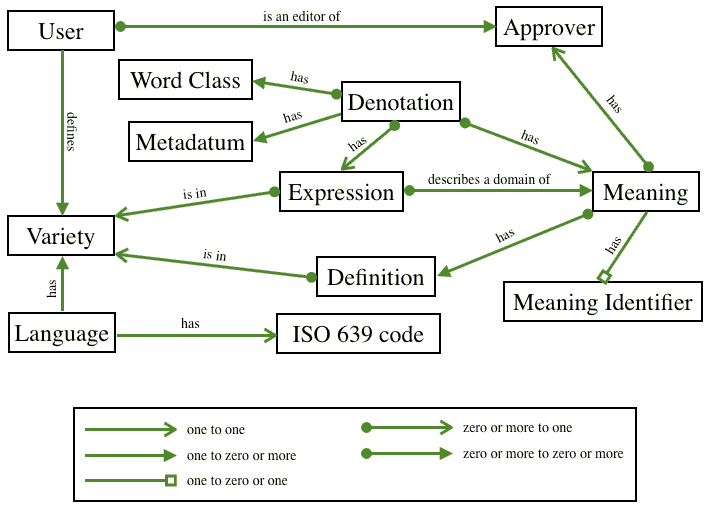
\includegraphics[width=0.4\textwidth]{images/schema.png}
\caption{The PanLex database schema}
\label{fig:db-schema}
\end{figure}

\begin{itemize}
  \item \emph{Expressions} are lemmas. For example, \emph{``go''} is a valid expression, whereas \emph{``went''} is not.
  Expressions are always given in a language variety and can only be given once per language variety.
  They were extracted from the afore mentioned mono- or bilingual dictionaries or from other sources.
  \item \emph{Languages} in PanLex are identified using ISO 639-3\footnote{\url{http://www.sil.org/iso639-3/codes.asp}} individual and macrolanguage codes, ISO 639-2\footnote{\url{http://www.loc.gov/standards/iso639-2/}} collective codes and ISO 639-5\footnote{\url{http://www.loc.gov/standards/iso639-5/}} codes.
  \item \emph {Language Varieties} within a language are further distinguished by arbitrary unique integer identifiers.
  For example, ``eng'' is the ISO 639-3 code for the English language.
  Panlex defines various varieties of it, including ``English'' (eng-000), ``Simple English'' (eng-001) and ``British English'' (eng-005).
  Their labels, when possible, are autonyms, written in the native writing system.
  So, in contrast to mechanisms like IETF BCP 47\footnote{\url{http://tools.ietf.org/html/bcp47}} there is no need for a transcription. %  and one can use variety names like ``{زبان اوستایی}''.
  Additionally these variety identifiers and labels do not have to be registered like the IETF BCP 47 language subtags\footnote{\url{http://www.iana.org/assignments/language-subtag-registry}}.
  \item \emph{Meanings} of expressions are distinguished by editors based on their
  interpretation of an information source.
%  Information sources can be dictionaries, thesauri, etc., and also personal knowledge. 
  The pair comprised of the editor and the information source is referred to as a meaning's \emph{approver}.
  Editors may add informal definitions to meanings in any language variety.
  \item \emph{Definitions} are optional descriptions of a meaning.
  They are given in a certain language variety.
  A description of the verb \emph{browse} for example could be \emph{``move or surf through various files on a computer, the Internet, etc.''}, marked as a definition in the ``English'' language variety.
  \item \emph{Denotations} relate expressions to meanings.
  So homonyms are represented by one expression being connected to different meanings.
  Denotations may be enriched with part-of-speech tags selected from a closed list based on the
  Open Lexicon Interchange Format (OLIF) standard\footnote{\url{http://www.olif.net/}}.
  For example, \emph{fall} can be a verb or a noun for autumn.
  Furthermore, it is possible to generically tag denotations with metadata
  using key-value pairs.
  For instance, an English expression \emph{pig} when synonymous with
  \emph{police officer} could be annotated with \emph{pragmatics=vulgar}.
  \item \emph{Users} have editorial privileges over the language varieties and the approvers that they define.
  \item \emph{Licenses} are also considered by the PanLex project.
  At present there are ten different license categories an approver can be annotated with.
  They are \emph{public domain}, \emph{Creative Commons}, \emph{request} (meaning that one has to ask the author of the resource), \emph{GNU General Public License}, \emph{GNU Lesser General Public License}, \emph{GNU Free Documentation License}, \emph{MIT License}, \emph{copyright} (stating that there is a certain copyright holder), \emph{other} and \emph{unknown}.
\end{itemize}

An overview of the number of instances per entity in the current PanLex database is given in~\autoref{fig:plx-entity-counts}.
\begin{table}
\centering
\begin{scriptsize}
\begin{tabular}{lr}
\toprule
Entity & Instances \\
%\midrule
Expressions & 18,580,594 \\ % SELECT COUNT(ex) FROM ex;
%\midrule
Languages   & 7,839 \\ % SELECT COUNT(lc) FROM lc; -- all language codes (ISO 639-3, ISO 639-2, ISO 639-5) known in the PanLex db
% FIXME: there should not be more languages than language varieties
%\midrule
Language Varieties & 7,248 \\ % SELECT COUNT(lv) FROM lv;
%\midrule
Meanings    & 20,023,427 \\ % SELECT COUNT(mn) FROM mn;
%\midrule
Definitions & 2,522,605 \\ % SELECT COUNT(df) FROM df;
%\midrule
Denotations & 50,803,243 \\ % SELECT COUNT(dn) FROM dn;
%\midrule
Users       & 7 \\ % SELECT COUNT(us) FROM us;
%\midrule
Licenses    & 10 \\ % SELECT COUNT(li) FROM apli;
\bottomrule
\end{tabular}
\end{scriptsize}
\caption{Number of entities in the PanLex database}
\label{fig:plx-entity-counts}
\end{table}


%\todo{Possibly also: approver editors, language variety editors, exemplar/approved characters, approver varieties}

%The same expression may be mentioned in multiple information sources.
%However, an expression's possible meanings depend on the user's interpretion of them in context of such a source.
%For this reason, every meaning depends on an approver.
%\emph{Denotations} capture the mappings between expressions and their possible meanings.  
Note that \emph{approver} combines a user with an \emph{information source},
however the \emph{information source} is not modelled as a distinct entity.
Also, the information of whether two meanings with different approvers
are still equal is not being captured. 


%These sources are fundamental for the PanLex database design and are aggregated in the approver table.
%According to these approvers there are special meanings that are represented by expressions.
%%Meanings are always related to an approver, which captures how a user interprets an expression information source.

%So, if there are two expressions, they can either be synonyms (if they are given in the same language) or translations of each other.
%\\
%Expressions are lexemes that can be seen as entries of a lexicon or dictionary of a given language.
%They are represented in their lemma or dictionary form.


%These expressions can be given in different language varieties allowing a meaning preserving translation between these varieties.
%An expression is given in a language variety.
%Such a variety can be a standard variety, a dialect, a script-based variety a controlled technical variety etc.
%Examples would be English, Simple English, British English and American English.\\


%  Ghidorah, the Three-Headed Monster | Ghidorah
%  describe or draw attention to (a product, service, or event) in a public medium in order to promote sales or attendance | advertise
%  move or surf through various files on a computer, the Internet, etc. | browse

\subsection{The PanLex vocabulary}
\label{sec:vocabulary}
%The schema described above was adopted to create RDF triple structures.
%is a good starting point most of the relations were taken over introducing a PanLex RDF vocabulary.
The entities and relations of the schema described in the previous section
serve as the base for the development of the PanLex RDF vocabulary.
In general, all PanLex RDF resources reside
in the namespace \texttt{<http://panlex.org/plx/>}, abbreviated with \texttt{plx}.
An example of the resulting ontology is depicted in \autoref{tbl:vocabulary} and
summarized as follows:
Unless otherwise noted, the URIs of instances of PanLex classes follow the pattern
\emph{plx:\{className\}/\{id\}}, where \{className\} is spelled in lower camel case
and the \{id\} is the primary key of the corresponding database table.

%As in the original PanLex database there are also \emph{expressions} used in the RDF dataset.
\begin{itemize}
\item Expressions are modeled as intances of \vocab{plx:Expression}.
Their textual representations and normalized versions thereof become the 
values of the properties \texttt{rdfs:label} and \texttt{plx:degradedText}, respectively.
Their corresponding language variety is stated
using \texttt{plx:languageVariety}.

\item For language and language varieties the classes
\texttt{plx:Language} and \texttt{plx:LanguageVariety} are introduced.
\emph{ISO 639-1} and \emph{ISO 639-3 codes} are of the classes
\texttt{plx:Iso639-1Code} and \texttt{plx:Iso639-3Code} respectively.

\item The RDF analog of the PanLex \emph{meaning} is the \texttt{plx:Meaning}.
Entities of this class may have an identifier assigned with the
\texttt{plx:identifier} property pointing to an \texttt{xsd:string} literal.
This meaning identifier represents ids given to the considered meaning in other
data sources and may at a later stage be used to build links to the meaning
as represented on these sites.
Meanings may also have \emph{definitions}, entities of the
\texttt{plx:Definition} class, giving a textual representation
(\texttt{rdfs:label}) with more than just a lexeme in a certain
language variety (\texttt{plx:languageVariety}).

%These resources have an \texttt{rdfs:label} containing the textual representation of the considered expression.
%Additionally there is a normalized version of the label, reachable via the \texttt{plx:degradedText} property.
%Expression entities also have an assigned language variety (\texttt{plx:languageVariety}).
%It refers to the language variety the textual representation is written in.
\item Following the semantics of the PanLex database, meanings and expressions are linked via \emph{denotations}.
These are entities of the \texttt{plx:Denotation} class pointing to meanings and expressions via the \texttt{plx:denotationMeaning} and \texttt{plx:denotationExpression} property respectively.
Denotations may also have a word class assigned to them.
This can be achieved with the denotation's \texttt{plx:wordClass} property pointing to a \texttt{plx:WordClass} entity.
\item All approvers share the \texttt{plx:Approver} class. The characteristics of an approver are described using mainly triples with literal objects.
These are for example \texttt{plx:registrationDate} pointing to an \texttt{xsd:date} literal,
\texttt{dc:title} to assign the title of a source,
\texttt{dc:creator} to give an \texttt{xsd:string} containing the author's name.
\end{itemize}

%These entities are mainly used for interlinking to the Lexvo dataset\footnote{\url{http://lexvo.org/ontology}}.
%See \autoref{sec:linking} for more details.



%Besides the approvers there are also \emph{languages} and \emph{language varieties} taken over into the RDF vocabulary.
%They are of the classes \texttt{plx:Language} and \texttt{plx:LanguageVariety} respectively.
%Language varieties have a name given by the \texttt{rdfs:label} property and belong to a certain language referred to via \texttt{plx:languageVarietyOf}.
%For those languages that have an ISO 639-3 language code, this code is referenced via the \texttt{plx:iso639-3Code} property.
%The equivalent ISO 639-1 code can be retrieved using the \texttt{plx:iso639-1Code} property.

%The structure of \emph{approvers} is nearly the same as in the database schema.
% etc.
%All properties defined for \texttt{plx:Approver} instances are shown in \autoref{tbl:vocabulary}.

%Besides the approvers there are also \emph{languages} and \emph{language varieties} taken over into the RDF vocabulary.
%They are of the classes \texttt{plx:Language} and \texttt{plx:LanguageVariety} respectively.
%Language varieties have a name given by the \texttt{rdfs:label} property and belong to a certain language referred to via \texttt{plx:languageVarietyOf}.
%For those languages that have an ISO 639-3 language code, this code is referenced via the \texttt{plx:iso639-3Code} property.
%The equivalent ISO 639-1 code can be retrieved using the \texttt{plx:iso639-1Code} property.

Since the PanLex project compiled its database by extracting data from different sources, the licenses of these sources were also considered.
At present, we support the different license categories given in the database by creating resources of the \texttt{plx:License} class.
%with appropriate descriptions in their \texttt{rdfs:label}.
%In the RDF dataset these have an additional \texttt{rdfs:label} property giving the names or descriptions 
\begin{table}
\begin{scriptsize}
\begin{tabular}{ll}
Class & Properties \\
\toprule
\texttt{plx:Approver} & \texttt{plx:registrationDate} \\
                      & \texttt{rdfs:label} \\
                      & \texttt{foaf:homepage} \\
                      & \texttt{plx:isbn} \\
                      & \texttt{dc:creator} \\
                      & \texttt{dc:title} \\
                      & \texttt{dc:publisher} \\
                      & \texttt{plx:yearOfPublication} \\
                      & \texttt{plx:quality} \\
                      & \texttt{plx:license} \\
\midrule
\texttt{plx:Language}
                      & \texttt{plx:iso639-3Code} \\
                      & \texttt{plx:iso639-1Code} \\
\midrule
\texttt{plx:LanguageVariety}
                      & \texttt{plx:languageVarietyOf} \\
                      & \texttt{rdfs:label} \\
\midrule
\texttt{plx:Iso639-1Code} & \\
\midrule
\texttt{plx:Iso639-3Code} & \\
\midrule
\texttt{plx:Expression}
                      & \texttt{plx:languageVariety} \\
                      & \texttt{rdfs:label} \\
                      & \texttt{plx:degradedText} \\
\midrule
\texttt{plx:Meaning}
                      & \texttt{plx:approver} \\
                      & \texttt{plx:meaningDefinition} \\
                      & \texttt{plx:identifier} \\
\midrule
\texttt{plx:Definition}
                      & \texttt{plx:languageVariety} \\
                      & \texttt{rdfs:label} \\
\midrule
\texttt{plx:Denotation}
                      & \texttt{plx:denotationMeaning} \\
                      & \texttt{plx:denotationExpression} \\
                      & \texttt{plx:wordClass} \\
\midrule
\texttt{plx:WordClass}  
                      & \texttt{rdfs:label} \\
\midrule
\texttt{plx:License}  & \texttt{rdfs:label} \\
\bottomrule
\end{tabular}
\end{scriptsize}
\caption{Classes and properties used in the PanLex RDF vocabulary. Note that all \texttt{rdf:type} and \texttt{rdfs:label} properties have been omitted for brevity.}
\label{tbl:vocabulary}
\end{table}

%An overview of the PanLex vocabulary is shown in \autoref{fig:vocabulary}.%
\begin{figure}
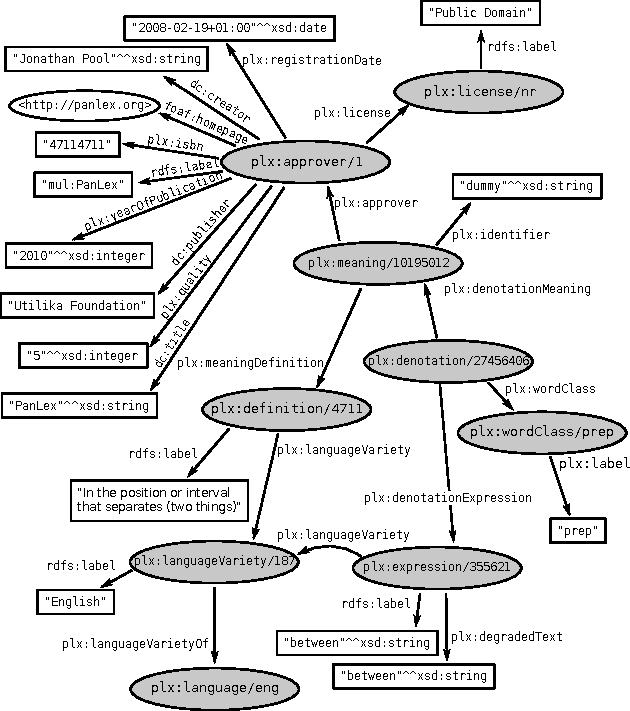
\includegraphics[width=0.47\textwidth]{images/pdf/ontology.pdf}
\caption{Overview of the PanLex RDF vocabulary}
\label{fig:vocabulary}
\end{figure}


\subsection{Transformation workflow}
\label{sec:conversion}
New sources are added to PanLex on almost a daily basis.   
The size of the PanLex database (including indexes) is currently approximately
18 GB, which is big enough to make recurrent RDF conversion cumbersome:
The RDF files of a full conversion of a dataset of this size are very huge.
Using conventional hardware, it takes impractically long
to convert all the data. This makes
testing and debugging and fixing issues in the modelling or data conversion of the
data very time-consuming.
As the PanLex data already resides in a relational database, the use of a virtual
RDB 2 RDF mapping solution is a natural choice. The \emph{Sparqlify Mapping Language}
offers a very easy-to-use mapping language.
Essentially, these mappings consist of three clauses:
\begin{itemize}
  \item \emph{From:} Specifies the logical SQL table (i.e. table, view or query) underlying the Sparqlify-ML view.
  \item \emph{With:} Defines SPARQL variables by means of expressions over relational columns that yield RDF terms.
  \item \emph{Construct:} The template (i.e. the set of triple patterns) to be generated in this view, based on the SPARQL variable definitions.
\end{itemize}
~\autoref{fig:ex:sparqlify-ml} shows an example of a Sparqlify-ML view for the
languages in PanLex: From each row of the \emph{i1} table three resources are
created from the \emph{iso3} column and 
bound to the variable names \emph{?lang}, \emph{?iso3} and \emph{?lexvo3}.
Resources for \emph{?lang} become typed as a \emph{Language} in the PanLex and the \emph{schema.org} namespace.
This view-based approach also demonstrates that changing the vocubulary or
adding support for new ones does not require an ETL process, and can therefore be done with little effort.
%\todo{Maybe we should link to lexvo directly.}
%PanLex's languages  iso 639-3 code 
%typed with plx:Language
%resources are created for
%the languages in PanLex, linked with \emph{lexvo}, and  
 
%how meanings are mapped to their definition text:
%Two resources are generated, namely \texttt{?mn} and \texttt{?mt}, which are typed with \texttt{plx:Meaning} and \texttt{plx:MeaningText} respectively.
%Note that we could not simply use \texttt{rdfs:label} for associating the definition text to the meaning resource directly, because
%the ISO 639-3 language code and PanLex language varieties do not directly map to valid RDF language tags.\todo{cite the standard} 
%Instead, we retained the variety information by attaching it to the meaning text resource.
%The with clause specifies the creation of URIs in the panlex namespace based on the respective entities database IDs.
%Furthermore, it defines the definition text to become a plain literal.

\begin{figure}
\centering
\begin{lstlisting}[basicstyle=\footnotesize\ttfamily]
Create View i1 As
  Construct {
    ?lang a plx:Language ;
          a <http://schema.org/Language> ;
          plx:iso639-3Code ?iso3 .

    ?iso3 a plx:Iso639-3Code ;
          owl:sameAs ?lexvo3 .
  }
  With
    ?lang = uri(concat(plx:language, '/', ?iso3))
    ?iso3 = uri(concat(plx:iso639-3, '/', ?iso3))
    ?lexvo3 = uri(concat('http://lexvo.org/id/iso639-3/', ?iso3))
  From
    i1
\end{lstlisting}
\caption{An excerpt of a Sparqlify-ML view definition for PanLex's languages. This
example also demonstrates how ``is-a relations'' to schema.org and links to lexvo are established.}
\label{fig:ex:sparqlify-ml}
\end{figure}


\section{Linking}
\label{sec:linking}
In this section we first describe how we interlinked PanLex's language codes
with Lexvo\footnote{\url{http://www.lexvo.org/}} and the expressions with DBpedia\footnote{\url{http://dbpedia.org}}.
Afterwards we give an overview of how the dataset and the related resources are published.

Since Lexvo covers all ISO 639-3 language codes, interlinking could be done with
the Sparqlify-ML view in Figure~\ref{fig:ex:sparqlify-ml}.
For DBpedia we were interested in creating \emph{valid} and
thus \emph{dereferenceable} links.
Therefore, we iterated the \emph{titles} datasets\footnote{\url{http://wiki.dbpedia.org/Downloads38} - Note that more languages are available in the raw download section at \url{http://downloads.dbpedia.org/3.8/}},
which map (non-localized) DBpedia URIs to their page titles in the respective language.
For each language version we normalized the labels: 
Unicode NFKD\footnote{\url{http://unicode.org/reports/tr15/}} normalization and
removal of punctuation characters were applied.
% PanLex now uses NFC, not NFKD, for character normalization and does not remove punctuation.
The DBpedia resources were then mapped to the PanLex expression that was equal to the resource's normalized label in the respective language.
Table ~\ref{fig:plx-dbp-link-counts} summarizes the number of links obtained.
\begin{table}
\centering
\begin{scriptsize}
\begin{tabular}{llll}
\toprule
Language & 639-1 & 639-3 & Links \\
\midrule
English    & en & eng & 1,415,241 \\
German     & de & deu &   224,146 \\
French     & fr & fra &   187,364 \\
Italian    & it & ita &   147,485 \\
Spanish    & sp & spa &   117,056 \\
Portuguese & pt & por &   112,266 \\
Polish     & pl & pol &   110,974 \\
Russian    & ru & rus &    68,040 \\
Czech      & cs & ces &    28,767 \\
Catalan    & ca & cat &    27,779 \\
Korean     & ko & kor &    24,912 \\
Turkish    & tr & tur &    22,258 \\
Bulgarian  & bg & bul &    19,431 \\
Hungarian  & hu & hun &    18,203 \\
Slovene    & sl & slv &    11,981 \\
Greek      & el & ell &     1,112 \\
\midrule
Total      &    &     & 2,537,015 \\
\bottomrule
\end{tabular}
\end{scriptsize}
\caption{Number of DBpedia links per language}
\label{fig:plx-dbp-link-counts}
\end{table}


% // (i1)
% // ISO 639-3 language name links to lexvo.org
% Create View i1 As
%     Construct {
%         ?iso1 a plx:Iso639-1Code.
%         ?iso3 a plx:Iso639-3Code.
%         ?iso1 owl:sameAs ?lexvo1.
%         ?iso3 owl:sameAs ?lexvo3.
%         ?lang a plx:Language.
%         ?lang a lvont:Language.
%         ?lang a <http://schema.org/Language>.
%         ?lang plx:iso639-1Code ?iso1.
%         ?lang plx:iso639-3Code ?iso3.
%     }
%     With
%         ?iso1 = uri(concat(plx:iso639-1, '/', ?iso1))
%         ?iso3 = uri(concat(plx:iso639-3, '/', ?iso3))
%         ?lexvo1 = uri(concat('http://lexvo.org/id/iso639-1/', ?iso1))
%         ?lexvo3 = uri(concat('http://lexvo.org/id/iso639-3/', ?iso3))
%         ?lang = uri(concat(plx:language, '/', ?iso3))
%     From
%         i1
% 

\section{Publishing}
\label{sec:publishing}
PanLex itself already provides direct access to the PostgreSQL database for scientists,
several user interfaces\footnote{\url{http://panlex.org/try/}} and an
API\footnote{\url{http://panlex.org/tech/doc/api/}}.
%The usage of these interfaces is not restricted in order to make the provided lexical
%translations as accessible as possible.
With our RDF conversion work, we complement these interfaces with
the Linked Data
%\footnote{\url{http://panlex.org/plx/TODO}}
and the SPARQL
endpoint\footnote{\url{http://panlex.org/sparql} and \url{http://panlex.org/snorql}}.
An overview is shown in ~\autoref{fig:panlex-architecture}.
Our code for interlinking is
hosted on GitHub\footnote{\url{https://github.com/AKSW/PanLex-2-RDF}}.
The created linksets are hosted in the PanLex database and published together
with the other data using Sparqlify.

\begin{figure}
\centering
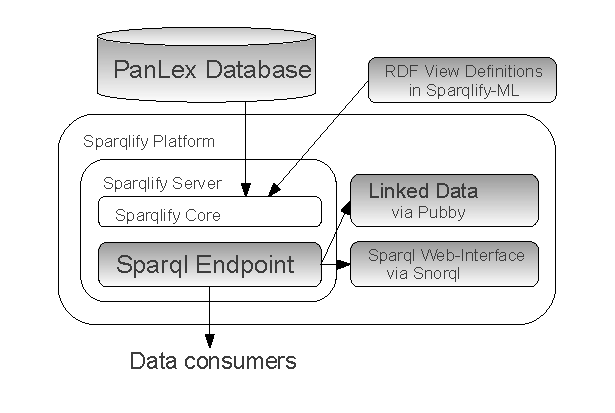
\includegraphics[width=0.4\textwidth]{images/PanLex-SW-Architecture}
\caption{PanLex architecture}
\label{fig:panlex-architecture}
\end{figure}

\todo{Fix the image: It should also show some sources which panlex uses.}


\section{Dataset Benefits and Usage Scenarios}
\label{sec:usage}
There are general benefits of RDF conversions,
such as the paradim shift towards thinking about what one intends to express
with the data, making this meaning explicit using ontologies,
enabling of interlinking, easing data integration tasks and uniform
data access via Linked Data and SPARQL.

With the RDF version of PanLex, a large lexical resource participates in the Web of Data,
making it available to a broader community. Users can easily explore the PanLex data using
the services provided by SNORQL and Pubby. This also increases the chance of development of
interesting mashups.
For example, the TeraDict translation service\footnote{\url{http://panlex.org/cgi-bin/apidemo-2.cgi}}
could be easily realized using simple SPARQL queries.
% as shown in
%\todo{Create the query: translations in a given target language of an expression}. 
Anothe future usage scenario is to link PanLex to Wortschatz in order to 
improve the recall of word-by-word translations by considering co-occurences.



\section{Related Work}
\label{sec:related}
PanLex is an integration project of many existing lexical resources with
the goal of eventually covering all languages in the world, especially
ones having few speakers.
The extraction of information from linguistic sources, and
techniques for automatically inferring translations, are
relevant work discussed in \cite{panlex_probtrans}. 

An important initiative is the
\emph{Global Wordnet Association}\footnote{\url{http://www.globalwordnet.org/}},
which offers a platform for sharing wordnets and defines several goals.
These include setting forth standards for uniformly representing wordnets
of different languages and establishing a universal index of meaning.

%It draws from the EuroWordNet~\cite{eurowordnet} and the  
%Manually engineered dictionaries %such as EuroWordNet [38]
% andcurrently mainly used for research purposes\todo{correct?}.
%A list of the resources used in panlex is compiled on the website\footnote{\url{http://panlex.org/tech/plrefs.shtml}}.
%In this section we discuss work related to the extraction and inference
%approaches used in PanLex, and work on the Semantic Web. 

%- There has been considerable research on methods to acquire translation lexicons from either
%MRDs (Neff and McCord, 1990; Helmreich et
%al., 1993; Copestake et al., 1994) or from par-
%allel text (Gale and Church, 1991; Fung, 1995;
%Melamed, 1997; Franz et al., 2001), but this has
%generally been limited to a small number of lan-
%guages.
%- Manually engineered dictionaries such as
%EuroWordNet (Vossen, 1998) (whats the name of the new project?)
%- TRANS GRAPH algorithm (Etzioni etal., 2007).

At the level of the Semantic Web, there is currently a trend in publishing linguistic resources
as Linked Data\footnote{\url{http://www.w3.org/DesignIssues/LinkedData.html}} and via SPARQL{\footnote{\url{http://www.w3.org/TR/sparql11-query/}}}.
These efforts are referred to as the \emph{Linguistic Linked Open Data Cloud} (LLOD)\footnote{\url{http://linguistics.okfn.org/resources/llod/}}. 
%Some of these datasets already make use of quasi-standard linguistic Semantic Web Ontolgies, such as  
Several (quasi-)standard ontologies have been developed for covering different aspects of linguistic resources.
Examples include the \emph{Ontologies of Linguistic Annotation} (OLiA)~\cite{olia2010},
the \emph{Lexicon Model for Ontologies} (lemon)~\cite{lemon2011} for modeling lexicon and machine-readable dictionaries,
\emph{POWLA} for modeling linguistic corpora\cite{powla2012}
and the \emph{Natural Language Processing Interchange Format} (NIF)\footnote{\url{http://nlp2rdf.org/nif-1-0}}.

%\begin{itemize}
%\item @author: Claus, Patrick
%\item Research related to PanLex itself \url{http://panlex.org/research/}
%\item Panlingual Translator: Word by word translation + back translation for verification, broken English (no grammar) ranked by
%Do we have a comparison to wiktionary?


%Difference to dict.cc\footnote{\url{http://dict.cc}}, leo.org\footnote{\url{http://leo.org}}, Wiktionary\footnote{\url{http://wiktionary.org}} and Wikipedia (DBpedia)


%\item 

%\item Research in the same field as PanLex
%\end{itemize}

\section{Conclusions and Future Work}
\label{sec:conclusion}
In this paper we describe the PanLex database and its conversion to RDF.
Based on our URI and vocabulary design, we created appropriate view definitions
for the virtual RDB to RDF solution \emph{Sparqlify} which carries out
the actual RDF transformation.
Furthermore, we interlinked the languages in PanLex with lexvo,
and created about 2.5 million links to DBpedia for expressions in 16 languages.
%We detailed the developed vocabulary and  

In this work we also identified some weaknesses in
the orginal database design,
which we intend to overcome in the future:
The orginal dataset currently does not cleanly model information sources and approvers
as distinct entities.
Also, while it is possible to determine each meaning's and each denotation's approver, an approver can have multiple users with editorial privileges, so it is not possible to track each contributed, modified, and deleted meaning and denotation by editor.
Retaining this information seems beneficial for translation approches,
as this enables for example the attribution of qualities and relevances to particular editors.

%\todo{Is there some quasi standard translation vocab we could re-use?}
%\todo{lang codes for minor languages}

\bibliographystyle{abbrv}
\bibliography{bibliography,../../bib/aksw}
\end{document}
